%%%%%%%%%%%%%%%%%%%%%%%%%%%%%%%%%%%%%%%%%
% Lachaise Assignment
% LaTeX Template
% Version 1.0 (26/6/2018)
%
% This template originates from:
% http://www.LaTeXTemplates.com
%
% Authors:
% Marion Lachaise & François Févotte
% Vel (vel@LaTeXTemplates.com)
%
% License:
% CC BY-NC-SA 3.0 (http://creativecommons.org/licenses/by-nc-sa/3.0/)
% 
%%%%%%%%%%%%%%%%%%%%%%%%%%%%%%%%%%%%%%%%%

%----------------------------------------------------------------------------------------
%	PACKAGES AND OTHER DOCUMENT CONFIGURATIONS
%----------------------------------------------------------------------------------------

\documentclass{article}

%%%%%%%%%%%%%%%%%%%%%%%%%%%%%%%%%%%%%%%%%
% Lachaise Assignment
% Structure Specification File
% Version 1.0 (26/6/2018)
%
% This template originates from:
% http://www.LaTeXTemplates.com
%
% Authors:
% Marion Lachaise & François Févotte
% Vel (vel@LaTeXTemplates.com)
%
% License:
% CC BY-NC-SA 3.0 (http://creativecommons.org/licenses/by-nc-sa/3.0/)
% 
%%%%%%%%%%%%%%%%%%%%%%%%%%%%%%%%%%%%%%%%%

%----------------------------------------------------------------------------------------
%	PACKAGES AND OTHER DOCUMENT CONFIGURATIONS
%----------------------------------------------------------------------------------------
\usepackage{listings}
\usepackage{amsmath,amsfonts,stmaryrd,amssymb} % Math packages
\usepackage{amsthm}

\usepackage{enumerate} % Custom item numbers for enumerations

\usepackage[linesnumbered,ruled,vlined]{algorithm2e} % Algorithms

\usepackage[framemethod=tikz]{mdframed} % Allows defining custom boxed/framed environments
\usepackage{subfigure}
\usepackage{listings} % File listings, with syntax highlighting
\usepackage{booktabs}
\usepackage{diagbox}

\lstset{
	basicstyle=\ttfamily, % Typeset listings in monospace font
}

%----------------------------------------------------------------------------------------
%	DOCUMENT MARGINS
%----------------------------------------------------------------------------------------

\usepackage{geometry} % Required for adjusting page dimensions and margins

\geometry{
	paper=a4paper, % Paper size, change to letterpaper for US letter size
	top=2.5cm, % Top margin
	bottom=3cm, % Bottom margin
	left=2.5cm, % Left margin
	right=2.5cm, % Right margin
	headheight=14pt, % Header height
	footskip=1.5cm, % Space from the bottom margin to the baseline of the footer
	headsep=1.2cm, % Space from the top margin to the baseline of the header
	%showframe, % Uncomment to show how the type block is set on the page
}

%----------------------------------------------------------------------------------------
%	FONTS
%----------------------------------------------------------------------------------------

\usepackage[utf8]{inputenc} % Required for inputting international characters
\usepackage[T1]{fontenc} % Output font encoding for international characters
% \usepackage{XCharter} % Use the XCharter fonts
\usepackage{CTEX}
\usepackage[hidelinks]{hyperref}

%----------------------------------------------------------------------------------------
%	COMMAND LINE ENVIRONMENT
%----------------------------------------------------------------------------------------

% Usage:
% \begin{commandline}
%	\begin{verbatim}
%		$ ls
%		
%		Applications	Desktop	...
%	\end{verbatim}
% \end{commandline}

\mdfdefinestyle{commandline}{
	leftmargin=10pt,
	rightmargin=10pt,
	innerleftmargin=15pt,
	middlelinecolor=black!50!white,
	middlelinewidth=2pt,
	frametitlerule=false,
	backgroundcolor=black!5!white,
	frametitle={Command Line},
	frametitlefont={\normalfont\sffamily\color{white}\hspace{-1em}},
	frametitlebackgroundcolor=black!50!white,
	nobreak,
}

% Define a custom environment for command-line snapshots
\newenvironment{commandline}{
	\medskip
	\begin{mdframed}[style=commandline]
}{
	\end{mdframed}
	\medskip
}

%----------------------------------------------------------------------------------------
%	FILE CONTENTS ENVIRONMENT
%----------------------------------------------------------------------------------------

% Usage:
% \begin{file}[optional filename, defaults to "File"]
%	File contents, for example, with a listings environment
% \end{file}

\mdfdefinestyle{file}{
	innertopmargin=1.6\baselineskip,
	innerbottommargin=0.8\baselineskip,
	topline=false, bottomline=false,
	leftline=false, rightline=false,
	leftmargin=2cm,
	rightmargin=2cm,
	singleextra={%
		\draw[fill=black!10!white](P)++(0,-1.2em)rectangle(P-|O);
		\node[anchor=north west]
		at(P-|O){\ttfamily\mdfilename};
		%
		\def\l{3em}
		\draw(O-|P)++(-\l,0)--++(\l,\l)--(P)--(P-|O)--(O)--cycle;
		\draw(O-|P)++(-\l,0)--++(0,\l)--++(\l,0);
	},
	nobreak,
}

% Define a custom environment for file contents
\newenvironment{file}[1][File]{ % Set the default filename to "File"
	\medskip
	\newcommand{\mdfilename}{#1}
	\begin{mdframed}[style=file]
}{
	\end{mdframed}
	\medskip
}

%----------------------------------------------------------------------------------------
%	NUMBERED QUESTIONS ENVIRONMENT
%----------------------------------------------------------------------------------------

% Usage:
% \begin{question}[optional title]
%	Question contents
% \end{question}

\mdfdefinestyle{question}{
	innertopmargin=1.2\baselineskip,
	innerbottommargin=0.8\baselineskip,
	roundcorner=5pt,
	nobreak,
	singleextra={%
		\draw(P-|O)node[xshift=1em,anchor=west,fill=white,draw,rounded corners=5pt]{%
		Question \theQuestion\questionTitle};
	},
}

\newcounter{Question} % Stores the current question number that gets iterated with each new question

% Define a custom environment for numbered questions
\newenvironment{question}[1][\unskip]{
	\bigskip
	\stepcounter{Question}
	\newcommand{\questionTitle}{~#1}
	\begin{mdframed}[style=question]
}{
	\end{mdframed}
	\medskip
}

%----------------------------------------------------------------------------------------
%	WARNING TEXT ENVIRONMENT
%----------------------------------------------------------------------------------------

% Usage:
% \begin{warn}[optional title, defaults to "Warning:"]
%	Contents
% \end{warn}

\mdfdefinestyle{warning}{
	topline=false, bottomline=false,
	leftline=false, rightline=false,
	nobreak,
	singleextra={%
		\draw(P-|O)++(-0.5em,0)node(tmp1){};
		\draw(P-|O)++(0.5em,0)node(tmp2){};
		\fill[black,rotate around={45:(P-|O)}](tmp1)rectangle(tmp2);
		\node at(P-|O){\color{white}\scriptsize\bf !};
		\draw[very thick](P-|O)++(0,-1em)--(O);%--(O-|P);
	}
}

% Define a custom environment for warning text
\newenvironment{warn}[1][Warning:]{ % Set the default warning to "Warning:"
	\medskip
	\begin{mdframed}[style=warning]
		\noindent{\textbf{#1}}
}{
	\end{mdframed}
}

%----------------------------------------------------------------------------------------
%	INFORMATION ENVIRONMENT
%----------------------------------------------------------------------------------------

% Usage:
% \begin{info}[optional title, defaults to "Info:"]
% 	contents
% 	\end{info}

\mdfdefinestyle{info}{%
	topline=false, bottomline=false,
	leftline=false, rightline=false,
	nobreak,
	singleextra={%
		\fill[black](P-|O)circle[radius=0.4em];
		\node at(P-|O){\color{white}\scriptsize\bf i};
		\draw[very thick](P-|O)++(0,-0.8em)--(O);%--(O-|P);
	}
}

% Define a custom environment for information
\newenvironment{info}[1][Info:]{ % Set the default title to "Info:"
	\medskip
	\begin{mdframed}[style=info]
		\noindent{\textbf{#1}}
}{
	\end{mdframed}
}
 % Include the file specifying the document structure and custom commands

%----------------------------------------------------------------------------------------
%	ASSIGNMENT INFORMATION
%----------------------------------------------------------------------------------------

\title{CS7304H: Statistical Learning\\Project
 Report} % Title of the assignment

\author{pangbo} % Author name and email address

\date{\today} % University, school and/or department name(s) and a date


%----------------------------------------------------------------------------------------

\begin{document}

\maketitle % Print the title

\section{数据}

本次的实验数据来自于一个文本分类数据集,这些样本被分类到20个不同的类别中。原始文本已经进行了特征提取预处理,每个样本为一个10000维向量。数据集分为训练数据与测试数据,训练数据包含11314个样本,测试数据包含7532个样本。

特征提取处理后的数据具有极高的稀疏度,训练数据与测试数据中分别约有$99.15\%$与$99.17\%$的元素为0。

从10000个特征维度来看:对于训练数据集,每个维度平均有95.6个非零元素,最多5272个非零元素,最少的维度没有非零元素,维度之间非零元素个数的方差为46729;对于测试数据集,每个维度平均有62.2个非零元素,最多3546个非零元素,最少的维度没有非零元素。特征维度非零元素个数的分布如图\ref{fig:dim-nnz}所示。

\begin{figure}[htbp]
    \centering
    \subfigure[训练数据集]{
        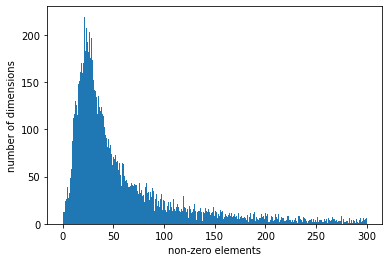
\includegraphics[width=0.44\linewidth]{figure/fig-train-dim-nonzero.png}
    }
    \hspace{0.5cm}
    \subfigure[测试数据集]{
        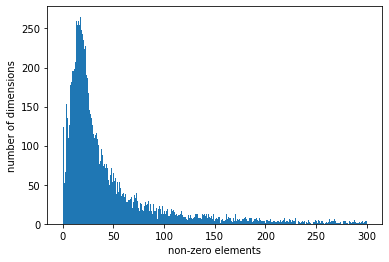
\includegraphics[width=0.44\linewidth]{figure/fig-test-dim-nonzero.png}
    }
    \caption{特征维度非零元素数分布}
    \label{fig:dim-nnz}
\end{figure}


从样本的角度看:对于训练数据集,平均每个样本有84.5个非零维度,单个样本最多有1600个非零维度,最少6个非零维度,非零维度数方差为8635;对于测试数据集,平均每个样本有82.6个非零维度,单个样本最多有1600个非零特征维度,最少3个非零维度。样本非零特征维度数的分布如图\ref{fig:sample-nnz}所示。

\begin{figure}[htbp]
    \centering
    \subfigure[训练数据集]{
        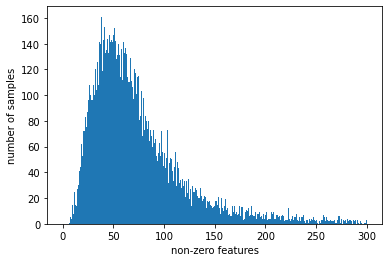
\includegraphics[width=0.44\linewidth]{figure/fig-train-sample-nonzero.png}
    }
    \hspace{0.5cm}
    \subfigure[测试数据集]{
        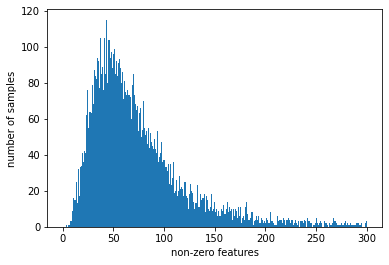
\includegraphics[width=0.44\linewidth]{figure/fig-test-sample-nonzero.png}
    }
    \caption{样本非零特征数分布}
    \label{fig:sample-nnz}
\end{figure}

训练数据的标签分布如图\ref{fig:train-label}所示。可以看出,训练数据的标签分布较为均匀,类别不平衡问题不明显,我们可以近似认为所有类别的先验概率是一致的。

\begin{figure}[h!]
    \centering
    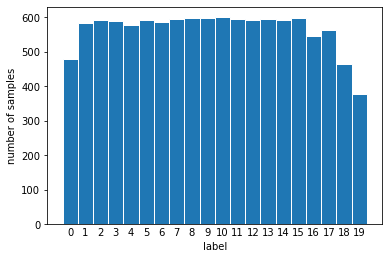
\includegraphics[width=0.5\linewidth]{figure/fig-labels.png}
    \caption{训练数据标签分布}
    \label{fig:train-label}
\end{figure}

为了更好展现数据的特征,我们分别使用t-SNE算法与PCA算法将数据降维到二维空间,降维结果如图\ref{fig:low-dim-visual}所示。图中每一个点代表训练集中的一个样本,点的颜色代表其所属的分类。从低维来看,这个分类问题是较为复杂甚至完全不可分的。

\begin{figure}[h!]
    \centering
    \subfigure[t-SNE]{
        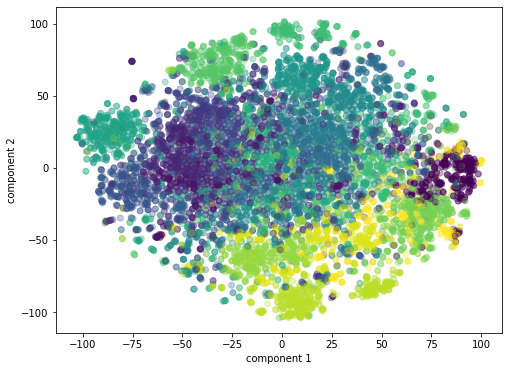
\includegraphics[width=0.44\linewidth]{figure/fig-tsne.png}
    }
    \hspace{0.5cm}
    \subfigure[PCA]{
        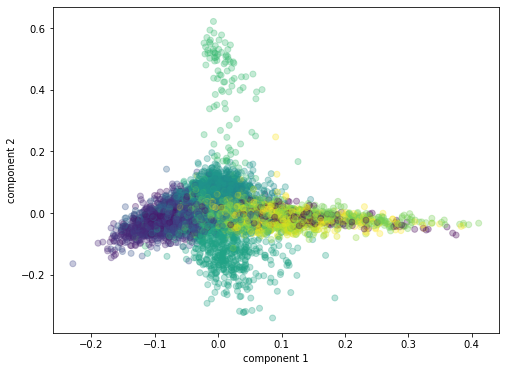
\includegraphics[width=0.44\linewidth]{figure/fig-pca.png}
    }
    \caption{样本降维可视化}
    \label{fig:low-dim-visual}
\end{figure}

\section{模型} % Unnumbered section

\subsection{SVM}

支持向量机(Support Vector Machine, SVM)是一种二分类模型,它的基本模型是定义在特征空间上的间隔最大的线性分类器,间隔最大使它有别于感知机;将SVM与核方法结合,SVM也可以用来求解非线性模型。

SVM优化问题可以表示为一个约束优化问题:
\begin{equation}
\begin{aligned}
\min_{w,b} \quad & \frac{1}{2}||w||^2 \\
s.t. \quad & y_i(w^Tx_i+b) \geq 1, \quad i=1,2,\cdots,n
\end{aligned}
\label{eq:svm-conopt}
\end{equation}

对于一个实际问题,直接求解问题\ref*{eq:svm-conopt}是非常困难的。首先,输入$x$维度可能是极高的,其次由于约束条件$y_i(w^Tx_i+b) \geq 1$的存在,这个问题可能不存在解,也就是我们的数据集在数学上可能不是线性可分的。

为了解决这个问题,我们可以使用利用罚函数法,将约束条件转化为目标函数的惩罚项,从而将约束优化问题转化为无约束优化问题。

\begin{equation}
\min_{w,b} \quad \frac{1}{2}||w||^2 + C\sum_{i=1}^n \max\left\{0, 1-y_i(w^Tx_i+b)\right\}
\label{eq:svm-unconopt}
\end{equation}

优化问题\ref{eq:svm-unconopt}中$C$是一个超参数,用来控制惩罚项的权重。当$C$趋于无穷大时,惩罚项的权重趋于无穷大,约束条件变为严格限制,此时目标函数的最优解就是问题\ref{eq:svm-conopt}的最优解。需要注意的是问题\ref{eq:svm-unconopt}的解不一定满足问题\ref{eq:svm-conopt}的约束条件,这表明训练得到的SVM可能会误分类部分训练数据点,在本场景下,我们可以容忍这种情况的出现。

为了优化问题\ref{eq:svm-unconopt},我们可以使用梯度下降法,算法伪代码如算法\ref{alg:svm-opt}所示。

\begin{algorithm}[]
    \label{alg:svm-opt}
    \DontPrintSemicolon
    \SetAlgoLined
    \KwIn{Train dataset $D=\{(x_1,y_1),(x_2,y_2),\cdots,(x_n,y_n)\}$, Learning rate $\eta$, Penalty factor $C$}
    \KwOut{ SVM parameters $w,b$}
    Initialize $w=0,b=0$\;
    \While{}{
        \For{$i=1,2,\cdots,n$}{
            \uIf{$y_i(w^Tx_i+b) < 1$}{
                $w \leftarrow w - \eta w + \eta C y_i x_i$\;
                $b \leftarrow b + \eta C y_i$\;
            }
            \Else{
                $w \leftarrow w - \eta w$\;
            }
        }
    }
    \caption{SVM优化算法}
\end{algorithm}

单个SVM只能进行二分类,为了实现多分类,需要将多个SVM进行组合,常用的方法有One-vs-One和One-vs-Rest两种:

\begin{enumerate}
    \item One-vs-One:对于$K$个类别,训练$K(K-1)/2$个SVM,每个SVM只对两个类别进行分类,预测时,将输入样本输入到所有的SVM中,选择获得最多正样本的类别作为预测结果。
    \item One-vs-Rest:对于$K$个类别,训练$K$个SVM,每个SVM只对一个类别进行分类。训练时,将这个类别的样本作为正样本,其他类别的样本作为负样本。预测时,将输入样本输入到所有的SVM中,选择输出最大的类别作为预测结果。
\end{enumerate}

由于本文的数据集有20个分类,One-vs-One方法需要训练190个SVM,而One-vs-Rest方法只需要训练20个SVM,因此我们考虑使用One-vs-Rest方法。

\subsection{Logistic Regression}

逻辑回归(Logistic Regression)是一种广义的线性回归模型。对于二分类问题,其形式为:

\begin{equation}
P(Y=1|x) = \frac{e^{w^Tx+b}}{1+e^{w^Tx+b}}
\label{eq:logistic-regression}
\end{equation}
逻辑回归可以较为容易地推广到多分类问题,对于$K$分类问题,其形式为:

\begin{equation}
P(Y=k|x) = \frac{e^{w_k^Tx+b_k}}{\sum_{i=1}^K e^{w_i^Tx+b_i}}
\label{eq:logistic-regression-multi}
\end{equation}

对分类问题,我们可以使用交叉熵损失函数计算预测损失:

\begin{equation}
L = -\sum_{i=1}^n \sum_{k=1}^K y_{ik}\log P(Y=k|x_i)
\label{eq:cross-entropy}
\end{equation}
基于交叉熵损失函数,我们可以使用梯度下降法优化模型参数$w,b$,其梯度为

\begin{equation}
\begin{aligned}
\frac{\partial L}{\partial w_k} &= -\sum_{i=1}^n x_i(y_{ik}-P(Y=k|x_i)) \\
\frac{\partial L}{\partial b_k} &= -\sum_{i=1}^n (y_{ik}-P(Y=k|x_i))
\end{aligned}
\label{eq:cross-entropy-gradient}
\end{equation}

优化算法伪代码如算法\ref{alg:logistic-regression-opt}所示。

\begin{algorithm}[]
    \label{alg:logistic-regression-opt}
    \DontPrintSemicolon
    \SetAlgoLined
    \KwIn{Train dataset $D=\{(x_1,y_1),(x_2,y_2),\cdots,(x_n,y_n)\}$, Learning rate $\eta$}
    \KwOut{ Logistic Regression parameters $w,b$}
    Initialize $w=0,b=0$\;
    \While{}{
        \For{$i=1,2,\cdots,n$}{
            $p_i\leftarrow \textsc{Softmax}(w^Tx_i+b)$\;
            $w \leftarrow w + \eta x_i(y_i-p_i)$\;
            $b \leftarrow b + \eta (y_i-p_i)$\;
        }
    }
    \caption{Logistic Regression优化算法}
\end{algorithm}

\subsection{神经网络}

全连接网络是最简单的神经网络结构,它的每个神经元都与前一层的所有神经元相连,形成一个密集的连接结构。全连接网络的每个神经元都有一个权重向量和一个偏置项,输入向量限于权重向量进行内积,加上偏置项,再通过激活函数进行非线性变换,便可以得到神经元的输出。

单层全连接网络可以表示成如下的数学形式:
\begin{align}
z^{(l)} = W^{(l)}a^{(l-1)} + b^{(l)}\\
a^{(l)} = f(z^{(l)})
\end{align}
其中$W^{(l)}$是第$l$层的权重矩阵,$b^{(l)}$是第$l$层的偏置向量,$f$是激活函数,$a^{(l)}$是第$l$层的输出向量。

神经网络可以通过反向传播算法进行训练:我们首先定义一个损失函数,然后让损失函数值对网络中的每个参数求偏导,得到每个参数的梯度,最后使用梯度下降法更新参数。对于分类问题,我们可以使用交叉熵损失函数计算预测损失,其函数形式已在公式\ref{eq:cross-entropy}中给出。

由于本场景下的问题并不算复杂,我们使用单个隐藏层的全连接网络进行拟合。

神经网络拥有众多参数,这导致模型有较高的过拟合风险。我们在隐藏层与输出层之间加入了Dropout层,Dropout层会随机地将一些神经元的输出置为0,从而减少神经元之间的依赖关系,防止过拟合。此外我们也将使用L2正则化,对模型的权重进行惩罚,抑制模型过拟合。


\section{模型选择}

模型选择旨在选出一个超参数集合,使得该超参数集合所代指的模型簇在指定问题上获得最好的泛化能力。

\subsection{Cross Validation}

交叉验证(Cross Validation)是一种统计学上将数据样本切分为训练集和测试集的方法。在交叉验证中,我们将数据集切分为$K$个大小相同的子集,每个子集都尽可能保持数据集的原始分布。然后我们依次将每个子集作为测试集,其他子集作为训练集,训练模型并计算模型在测试集上的性能。最后我们将$K$次测试结果的平均值作为模型的性能。

\subsection{Bootstrap}

自助法(Bootstrap)是一种统计学上用来估计统计量偏差的方法。在自助法中,我们从数据集中有放回地抽取$n$个样本,作为训练集,剩余的样本作为测试集,训练模型并计算模型在测试集上的性能。重复这个过程$K$次,最后我们将$K$次测试结果的平均值作为模型的性能。

相较于交叉验证,自助法允许数据放回,对于训练数据较少的场景,自助法可以更好地利用数据集。

\subsection{Grid Search}

网格搜索(Grid Search)是一种超参数优化方法。对于实际的机器学习问题,模型往往有多个超参数,超参数之间会互相影响,如果我们每次只对一个超参进行搜索,最终的组合结果并不一定是最优的。

在网格搜索中,我们首先选定每个超参数的取值范围,然后取笛卡尔积,也即穷举所有超参数的取值组合,对于每个超参数组合,使用交叉验证或者自助法计算模型的性能,最后选出性能最好的超参数组合。

\section{实验}

在实验部分,我们会比较不同模型的性能。对于每一种模型,我们首先会使用网格搜索找到性能最好的一组超参数,然后使用该组超参数在完整训练集上训练模型,用得到的模型预测测试集,提交预测结果获得测试分数。

在网格搜索中,对于每一组超参,我们使用5折交叉验证计算模型的性能。

\subsection{Logistic Regression}

逻辑回归拥有两个超参数:学习率与迭代轮数。对这两个超参数的搜索结果如表\ref{tab:lr-grid-search}所示。在所有的超参数组合中,学习率为100,训练轮数为1000时,模型获得了最好的性能,5折交叉验证的平均准确率为0.9020。

\begin{table}[htbp]
\label{tab:lr-grid-search}
\caption{Logistic Regression网格搜索结果}
\begin{center}
    \begin{tabular}{cccc}
        \toprule
        \diagbox{lr}{n\_iters}  &    500.0  &    1000.0 &    2000.0 \\
        \midrule
        0.1    &  0.4578 &  0.6419 &  0.7412 \\
        1.0    &  0.7970 &  0.8211 &  0.8422 \\
        10.0   &  0.8662 &  0.8854 &  0.8950 \\
        100.0  &  0.9004 &  \textbf{0.9020} &  0.9000 \\
        1000.0 &  0.8809 &  0.8802 &  0.8817 \\
        \bottomrule
    \end{tabular}
\end{center}
\end{table}

使用上述超参数在训练集上训练模型,预测测试集,提交预测结果,获得测试分数为0.83488,如图\ref{fig:submit-lr}所示。

\begin{figure}[htbp]
    \centering
    
\includegraphics[width=0.8\linewidth]{figure/fig-submit-lr.png}
    \caption{Logistic Regression测试分数}
    \label{fig:submit-lr}
\end{figure}

\subsection{SVM}

支持向量机拥有两个超参数:学习率与惩罚因子。对这两个超参数的搜索结果如表\ref{tab:svm-grid-search}所示。在所有的超参数组合中,学习率为$10^{-6}$,惩罚因子为$10^{5}$时,模型获得了最好的性能,5折交叉验证的平均准确率为0.9045。

\begin{table}[htbp]
\label{tab:svm-grid-search}
\caption{SVM网格搜索结果}
\begin{center}
    \begin{tabular}{ccccc}
        \toprule
        \diagbox{lr}{C} &  $10^{4}$    &  $10^{5}$   &  $10^{6}$  &  $10^{7}$ \\
        \midrule
        $10^{-7}$ &    0.8643 &    \textbf{0.9045} &    0.8972 &    0.8820 \\
        $10^{-6}$ &    0.8951 &    0.8975 &    0.8857 &    0.8751 \\
        $10^{-5}$ &    0.8867 &    0.8675 &    0.8122 &    0.7728 \\
        $10^{-4}$ &    0.7781 &    0.6021 &    0.5692 &    0.5667 \\
        \bottomrule
        \end{tabular}
\end{center}
\end{table}

使用上述超参数在训练集上训练模型,预测测试集,提交预测结果,获得测试分数为0.82267,如图\ref{fig:submit-svm}所示。

\begin{figure}[htbp]
    \centering
    
\includegraphics[width=0.8\linewidth]{figure/fig-submit-svm.png}
    \caption{SVM测试分数}
    \label{fig:submit-svm}
\end{figure}

\subsection{神经网络}

神经网络具有较多超参数,我们首先固定模型具有一个隐藏层,且训练中的学习率为$10^{-3}$,其余需要搜索的超参数包括:参数正则化系数、Dropout层的丢弃率、隐藏层的神经元个数、训练轮数。

对这些超参数的搜索结果如表\ref{tab:nn-grid-search}所示。表中参数的含义如下:
\begin{itemize}
    \setlength{\itemsep}{0pt}
    \setlength{\parsep}{0pt}
    \setlength{\parskip}{0pt}
    \item decay:Adam优化器的weight\_decay参数,等效于L2正则化的系数。
    \item drop:Dropout层的丢弃率,即在训练时屏蔽单个神经元输出的概率。
    \item hidden:隐藏层的神经元个数。
    \item epoch:训练轮数。
\end{itemize}

在所有的超参数组合中,参数正则化系数为$10^{-6}$,Dropout层的丢弃率为0.9,隐藏层的神经元个数为1024,训练轮数为20时,模型获得了最好的性能,5折交叉验证的平均准确率为0.9167。


\begin{table}[htbp]
    \label{tab:nn-grid-search}
    \begin{center}
        \caption{神经网络网格搜索结果}
        \begin{tabular}{cc|ccc|ccc|ccc}
            \toprule
            & hidden & \multicolumn{3}{c|}{1024} & \multicolumn{3}{c|}{1536} & \multicolumn{3}{c}{2048} \\
                         & epoch &   15 &   20 &   25 &   15 &   20 &   25 &   15 &   20 &   25 \\
                         \cline{1-2}
            decay & drop &        &        &        &        &        &        &        &        &        \\
            \hline
             & 0.7 & 0.9130 & 0.9135 & 0.9121 & 0.9123 & 0.9115 & 0.9118 & 0.9122 & 0.9121 & 0.9121 \\
             0 & 0.8 & 0.9144 & 0.9135 & 0.9121 & 0.9141 & 0.9129 & 0.9122 & 0.9125 & 0.9117 & 0.9129 \\
                         & 0.9 & 0.9146 & 0.9147 & 0.9142 & 0.9151 & 0.9152 & 0.9136 & 0.9136 & 0.9140 & 0.9135 \\
            \hline
             & 0.7 & 0.9129 & 0.9120 & 0.9132 & 0.9118 & 0.9121 & 0.9124 & 0.9128 & 0.9119 & 0.9123 \\
             $10^{-7}$  & 0.8 & 0.9141 & 0.9132 & 0.9128 & 0.9127 & 0.9118 & 0.9133 & 0.9126 & 0.9115 & 0.9131 \\
                         & 0.9 & 0.9129 & \textbf{0.9167} & 0.9149 & 0.9154 & 0.9135 & 0.9136 & 0.9144 & 0.9140 & 0.9136 \\
            \hline
             & 0.7 & 0.9129 & 0.9117 & 0.9113 & 0.9117 & 0.9113 & 0.9122 & 0.9117 & 0.9110 & 0.9107 \\
             $10^{-6}$  & 0.8 & 0.9130 & 0.9137 & 0.9122 & 0.9133 & 0.9121 & 0.9117 & 0.9113 & 0.9116 & 0.9119 \\
                         & 0.9 & 0.9142 & 0.9154 & 0.9152 & 0.9153 & 0.9142 & 0.9138 & 0.9146 & 0.9131 & 0.9121 \\
            \hline
             & 0.7 & 0.9109 & 0.9104 & 0.9087 & 0.9095 & 0.9086 & 0.9080 & 0.9080 & 0.9075 & 0.9068 \\
             $10^{-5}$ & 0.8 & 0.9123 & 0.9106 & 0.9101 & 0.9115 & 0.9099 & 0.9092 & 0.9099 & 0.9104 & 0.9080 \\
                         & 0.9 & 0.9141 & 0.9142 & 0.9126 & 0.9127 & 0.9129 & 0.9122 & 0.9142 & 0.9133 & 0.9104 \\
            \bottomrule
            \end{tabular}
    \end{center}
\end{table}

使用上述超参数在训练集上训练模型,预测测试集,提交预测结果,获得测试分数为0.85771,如图\ref{fig:submit-nn}所示。

\begin{figure}[htbp]
    \centering
    
\includegraphics[width=0.8\linewidth]{figure/fig-submit-nn.png}
    \caption{神经网络测试分数}
    \label{fig:submit-nn}
\end{figure}

\subsection{降维}

最后,我们还尝试使用PCA对特征进行降维,然后使用降维后的特征训练模型。

\begin{figure}[htbp]
    \centering
    
\includegraphics[width=0.8\linewidth]{figure/fig-submit-lr-pca.png}
    
\includegraphics[width=0.8\linewidth]{figure/fig-submit-nn-pca.png}
    
\includegraphics[width=0.8\linewidth]{figure/fig-submit-svm-pca.png}
    \caption{降维后测试分数}
    \label{fig:submit-pca}
\end{figure}

降维后的测试分数如图\ref{fig:submit-pca}所示。根据测验结果,使用PCA降维后训练结果并不理想,最终准确率不如使用原始数据训练的模型。我认为可能的原因在于PCA降维后,数据的可分性变差了,尤其是本实验中大多采用线性模型,只有对于足够稀疏的特征空间,线性决策边界才能将不同类别的样本分开,而PCA降维后,样本点分布变得紧密与复杂,导致线性模型的性能变差。

\end{document}
